\section{Astrophysical Sources of Gamma-rays}
\seclabel{astrophysical_sources}

\subsection{Pulsars}

It is widely accepted that in the collapse of a massive star, a large
amount of ejecta is released as a supernova powering a \ac{SNR}
and that much of the remaining mass collapses into a neutron star
\citep{baade_1934a_remarks-super-novae}.

Pulsars were first discovered observationally in 1967 by Jocelyn Bell
Burnell and Antony Hewish \citep{hewish_1968_observation-rapidly}. They
had constructed a radio telescope that used interplanetary scintillation
wiht the intention of observing quasars.  In the process, they
detected a source with a periodicity of 1.3 \second. We note in
passing that pulsars had been previously observed by the air force
\citep{brumfiel_2007_force-early}.

Even before the discovery, \cite{pacini_1967_energy-emission}
had predicted the existence of \acp{NS}.  Shortly following
the 1967 discovery, \cite{gold_1968_rotating-neutron} and
\cite{pacini_1968_rotating-neutron} argued that the observed pulsar was
a rotating \ac{NS}.

The discovery of many more pulsars came quickly.  In 1968, and the
Vela pulsar \citep{large_1968_pulsar-supernova} and the Crab pulsar
\citep{staelin_1968_pulsating-radio} were discovered.

The first pulsar observed at optical frequencies was the
Crab, discovered in 1969 shortly after its radio discvoery
\citep{cocke_1969_discovery-optical}.  In the same year, the first X-ray
pulsations were discovered from the same source. At the time, there were
no space-based X-ray observatories, so observations had to be performed
from rockets.  The discovery was carried out almost concurrently by
a group at \gls{NRL} \citep{fritz_1969_x-ray-pulsar} and at \gls{MIT}
\citep{bradt_1969_x-ray-optical}.  Using proportional counters, these
experiments showed that the pulsed emission from the Crab extended to
X-ray energies and that, for this source, the X-rays emission was a
factor $>100$ more energetic than the observed visible emission.

\begin{itemize}
  \item I read somewhere, but don't have the reference (it was one
    of htose verbose history books on pulsars), that originally
    the neutron star hypothesis wasn't well accepted. But then
    one pulsar was found with a very short period (I think the Crab)
    which, for causaility reasons, had to be small enough taht it
    seemed to confirm the Neutron star hypotehsis.
  \item For Crab describe spin down?: ``and these pulsations were then shown to be slowing down at a
    rate of 36 ns per day (Richards \& Comella 1969).'' -- \cite{gaensler_2006_evolution-structure}
\end{itemize}

As was discussed in \secref{history_gamma_ray_detectors},
$\gamma$-ray emission from the Crab was detected only 2 years
later \citep{browning_1971_detection-pulsed}.

\todo{First gamma-ray detection}

ATNF catalog?

\begin{itemize}
  \item ``There are currently more than 1,800 pulsars in the ATNF on-line
  catalog [Manchester et al., 2005], with rotation periods in the rage
  0.0016-12 seconds (Figure 3.1) and derived spin down
  luminosities in the range XXX - XXX erg/s.'' -- dalton\_2011\_identication-gamma-ray
\end{itemize}

EGRET pulsars?

The state of the art in $\gamma$-ray detection of pulsars
will be included in an upcomming pulbication.
2PC: \secref{second_pulsar_catalog}

\todo[inline]{When was the PSR, PWN connection made}


\subsection{\Acptitle{PWN}}

% Good history of observations of crab nebulae:
%  * chapter 1 of "The Crab Nebula" by Rodney Deane Davies

% Good history paper: ``Pulsar Wind Nebulae:
%   On their growing diversity and association
%   with highly magnetized neutron stars''
%   by Samar Safi-Harb
%   -- http://arxiv.org/pdf/1211.0852.pdf

% Good paper on Crab Nebula: ``{The Crab Nebula: An Astrophysical Chimera}'' by
%   J. Jeff Hester

% Good review of PWN: 
%   ``The Evolution and Structure of Pulsar Wind Nebulae''
%   Bryan M. Gaensler and Patrick O. Slane

% Good review of PWN:
%  ``{Pulsar Wind Nebulae in the Chandra Era}''
%  O. Kargaltsev and G. G. Pavlov


% lots of INFO on M1 (crab): http://messier.seds.org/m/m001.html


A \gls{PWN} is a diffuse nebula of shocked relativistic particles.
A \glspl{PWN} surrounds and is powered by an accompanying pulsar. 
\glspl{PWN} have been observed long before the discovery of pulsars, but
the pulsar/\gls{PWN} connection could not be made until
after the detection of pulsars.

The most famous \glspl{PWN} is the Crab nebula, associated with
the Crab pulsar.

\begin{itemize}
  \item Chinese SN observations of Crab Nebulae: (p128 of ``The Crab Nebula: An Astrophysical Chimera'')
     ``It was probably also recorded by Anasazi Indian artists (in
     present-day Arizona and New Mexico), as findings in Navaho Canyon and
     White Mesa (both Arizona) as well as in the Chaco Canyon National
     Park (New Mexico) indicate; there's a review of the research on
     the Chaco Canyon Anasazi art online. In addition, Ralph R. Robbins
     of the University of Texas has found Mimbres Indian art from New
     Mexico, possibly depicting the supernova.'' -- http://messier.seds.org/m/m001.html
\end{itemize}

It was discovered in
1731 by physician and amateur astronomer John Bevis.  This source was
going to be published in his sky atlas {\em Uranographia Britannica}, but
the work was never publisehd because his published filed for bankrupcy
in 1950.  Figure~\figref{bevis_crab} shows Beavis' plate containing
the Crab nebula.  A detailed history of John Bevis' work can be found
in \cite{ashworth_1981_bevis-uranographia}.


\begin{figure}[htbp]
  \centering
  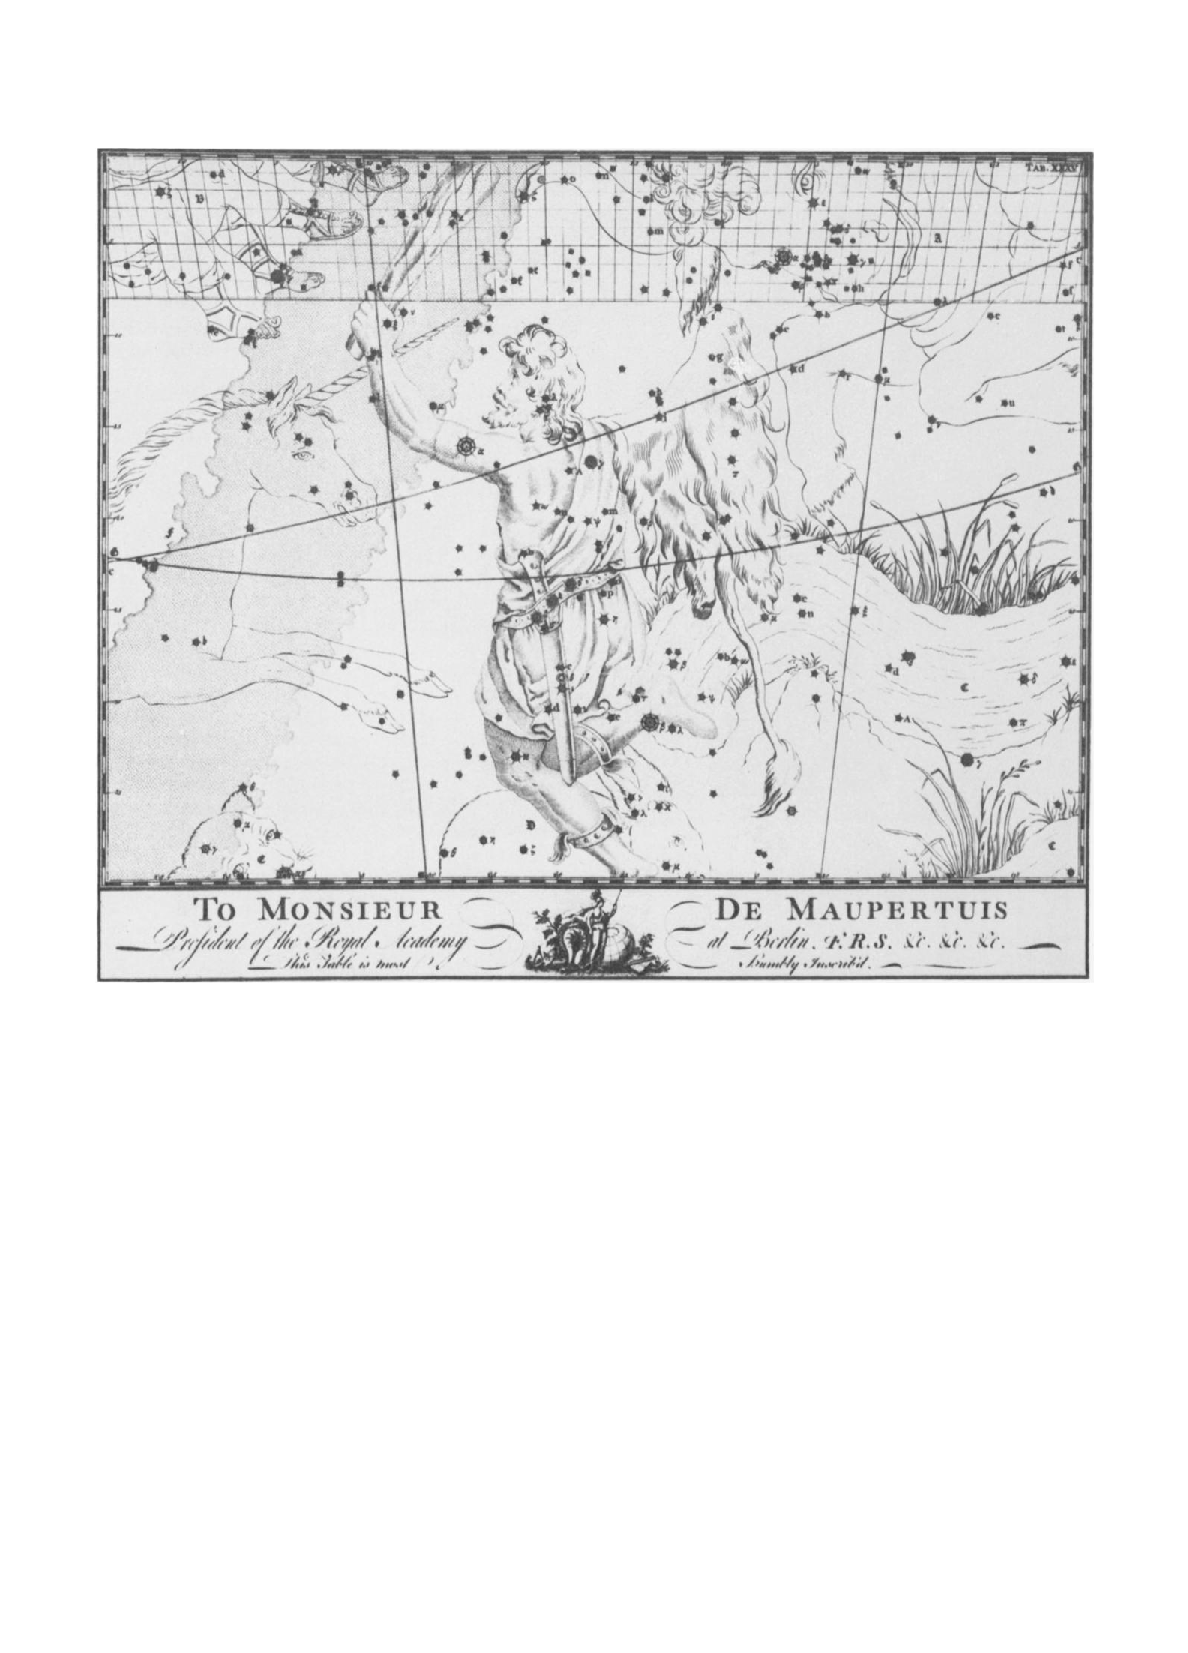
\includegraphics[width=\textwidth]{chapters/introduction/figures/bevis_crab.pdf}
  \figlabel{bevis_crab}
  \caption{The Orion plate from Bevis' book {\em Uranographia Britannica}.
  The Crab nebula can be found on the horn of Taurus the Bull 
  on the top of the figure and the source is marked by a 
  cloudy symbol.
  This figure was reproduced from \cite{ashworth_1981_bevis-uranographia}.}
\end{figure}

\begin{itemize}
  \item Crab Nebulae is M1 in Charles Messier's catalog 1758 
    (p128 of ``The Crab Nebula: An Astrophysical Chimera'')
  \item Connection to 1054:
    ``Lundmark (1921) suggested a connection between the Crab Nebula and the event of 1054 AD''
    (p128 of ``The Crab Nebula: An Astrophysical Chimera'')
    ``The Crab Nebula (Fig. 1) is almost certainly associated with a
    supernova (SN) ex- plosion observed in 1054 CE (Stephenson \& Green
    2002, and references therein).'' -- ``The Evolution and Structure of Pulsar Wind Nebulae'' 
    Bryan M. Gaensler and Patrick O. Slane
  \item ``The same year, J.C. Duncan of Mt. Wilson Observatory compared
    photographic plates taken 11.5 years apart, and found that the
    Crab Nebula was expanding at an average of about 0.2'' per year;
    backtracing of this motion showed that this expansion must have
    begun about 900 years ago (Duncan 1921). Also the same year, Knut
    Lundmark noted the proximity of the nebula to the 1054 supernova
    (Lundmark 1921).`` -- http://messier.seds.org/m/m001.html
    ``In 1942, based on investigations with the 100-inch Hooker telescope
    on Mt. Wilson, Walter Baade computed a more acurate figure of 760
    years age from the expansion, which yields a starting date around
    1180 (Baade 1942); later investigations improved this value to about
    1140. The actual 1054 occurrance of the supernova shows that the
    expansion must have been accelerated.'' -- http://messier.seds.org/m/m001.html
  \item ``but it was not until 1942 that Duyvendak (1942) and Mayall \&
  Oort (1942) presented complete studies of modern observations of the
  expanding nebula and of the early Chinese records. It was this work
  that established unambiguously that the Crab is the remnant of SN1054.''
    (p128 of ``The Crab Nebula: An Astrophysical Chimera'')
  \item ``1949, the Crab nebula was identified as a strong source
  of radio radiation (Bolton et.al. 1949), discovered 1948 named
  and listed as Taurus A (Bolton 1948), and later as 3C 144.'' -
  http://messier.seds.org/m/m001.html




  \item Synchrotron emission hypotehsis: ``while the inner, blueish
      nebula emits continuous light consisting of highly polarised so-called
      synchrotron radiation, which is emitted by high-energy (fast moving)
      electrons in a strong magnetic field. This explanation was first
      proposed by the Soviet astronomer J. Shklovsky (1953) and supported
      by observations of Jan H. Oort and T. Walraven (1956).'' -- http://messier.seds.org/m/m001.html
  \item ``X-rays from this object were detected in April 1963 with a
      high-altitude rocket of type Aerobee with an X-ray detector developed
      at the Naval Research Laboratory; the X-ray source was named Taurus
      X-1. Measurements during lunar occultations of the Crab Nebula on
      July 5, 1964, and repeated in 1974 and 1975, demonstrated that the
      X-rays come from a region at least 2 arc minutes in size, and the
      energy emitted in X-rays by the Crab nebula is about 100 times more
      than that emitted in the visual light''
        -- http://messier.seds.org/m/m001.html
  \item Association of Crab pulsar with Crab nebulae were 
    discussed in \citep{staelin_1968_pulsating-radio}.

\item
"Just after discovery of pulsars, Gunn \& Ostriker (1969) suggested
that particles can be accelerated to very high energies in the pulsar
wind zone." -- "Relativistic Astrophysics and Cosmology" by Shapiro


  \item TEV observations of Crab. brightest soruce in the sky\ldots
  \item Now many radio, x-ray PWNe. Count form PWN catalog: http://www.physics.mcgill.ca/~pulsar/pwncat.html
    ``Observations over the last several decades have identified 40 to 50
    further sources, in both our own Galaxy and in the Magellanic Clouds,
    with properties similar to those of the Crab Nebula (Green 2004;
    Kaspi, Roberts \& Harding 2006)'' -- \cite{gaensler_2006_evolution-structure}
  \item How many TeV PWNe in TeVCat? http://tevcat.uchicago.edu/ (31 by my preliminary count)
\end{itemize}




